% #############################################################################
% Chapter 2 - State of the Art
% !TEX root = ../main.tex
% #############################################################################

%\fancychapter{State of the Art}
\newfancychapter{State of the Art}{ %
This chapter presents the state of the art in the field of magnetoresistive sensors and their interfaces. It provides valuable information about the sensors utilized in this work, as well as an overview of the systems developed both within and outside of INESC that interface with these sensors. By including a comprehensive review of the state of the art in magnetoresistive sensors and their interfaces, this chapter establishes a solid foundation of knowledge to understand the subsequent chapters and support the development of an optimized interface for the magnetoresistive sensors.
}
\label{chapter:state-of-the-art}

% Uncomment before printing
\clearpage
%\thispagestyle{empty}
%\cleardoublepage

% #############################################################################
\section{Magnetoresistive Sensors}
\label{section:soa-mr-sensors}

\ac{MR} sensors are small components designed to sense an applied magnetic field. Their \ac{MR} effect occurs when the electrical conductor present in the sensor changes resistance based on an applied magnetic field. The resistance value may increase or decrease, depending on the orientation of the magnetic field \cite{Magnetor15:online}.

The \ac{MR} sensors were discovered in 1857 by Lord Kelvin that noticed a slight change in the electrical resistance of a piece of iron when he placed it in a magnetic field. Although the mechanism responsible for \ac{AMR} discovered by Kelvin and \ac{GMR} discovered by Grünberg \cite{PhysRevB.39.4828} and Fert \cite{PhysRevLett.61.2472} is different, both surge from the interaction of a current with the magnetism of the material \cite{Thompson_2008}. However, the \ac{GMR} phenomen is the most interesting for this project so it will be explained in detail in the next section. The cause of magnetism in a ferromagnetic material is the uneven distribution of electrons in atoms \cite{dionne2009magnetic}. That results in a spin-polarized band structure in which there is an imbalance in the number of spin-up and spin-down electrons and consequently net magnetization \cite{Thompson_2008}. The \ac{MR} sensors have linear change of their electrical resistance with magnetic fields.

Figure \ref{figure:mr-transfer-curves} illustrates the transfer curve that has two types, depending on the sensors. \ac{SV}, \ac{MTJ}, and planar Hall sensors have a response to an external magnetic field like Figure \ref{figure:mr-transfer-curves-a} with the linear region centered at $0T$. However, \ac{AMR} and \ac{GMR} multilayer sensors have a transfer curve like Figure \ref{figure:mr-transfer-curves-b} with the resistance value near $R_{max}$ at $0T$, meaning that it is required an external magnetic field to obtain their maximum linearity. 

\begin{figure}[!ht]
    \centering
    \begin{subfigure}[b]{.45\textwidth}
        \centering
        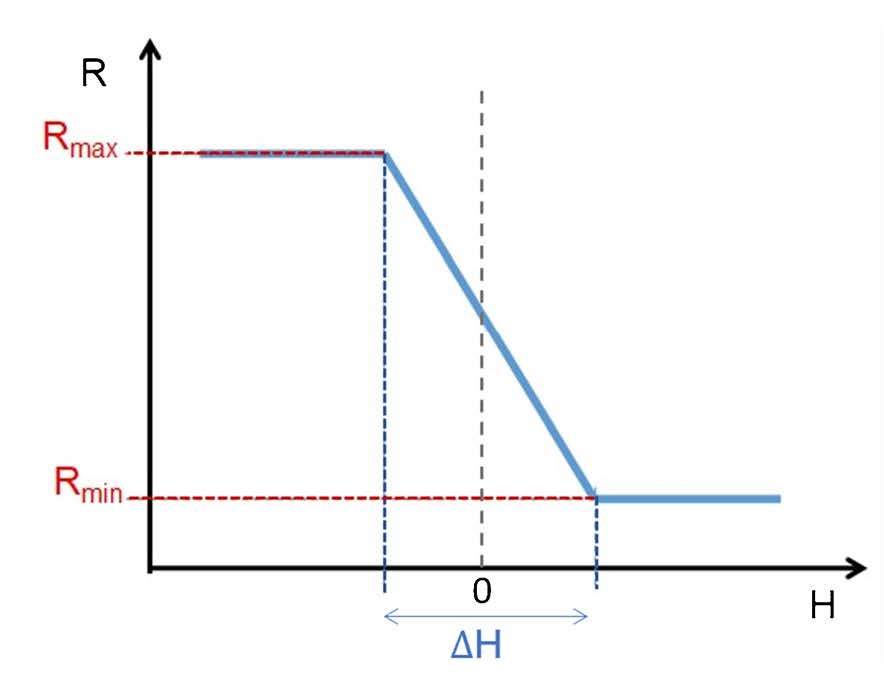
\includegraphics[width=.8\textwidth]{mr_transfer_curves_a.jpg}
        \caption{Spin valve, magnetic tunnel junctions, and planar Hall.}
        \label{figure:mr-transfer-curves-a}
    \end{subfigure}
    \hfill
    \centering
    \begin{subfigure}[b]{.45\textwidth}
        \centering
        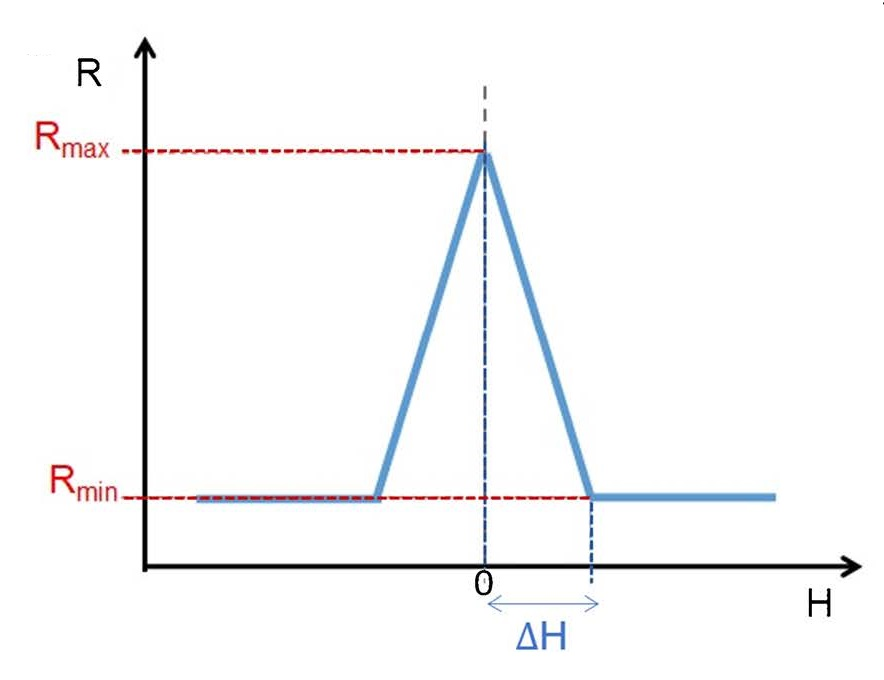
\includegraphics[width=.8\textwidth]{mr_transfer_curves_b.jpg}
        \caption{AMR and GMR multilayers.}
        \label{figure:mr-transfer-curves-b}
    \end{subfigure}
    \caption{Schematic of the linear MR sensors transfer characteristic (from Soares \textit{et al.} \cite{Soares2019}).}
    \label{figure:mr-transfer-curves}
\end{figure}

The performance of the sensors depends on the magnetoresistance ratio and sensitivity. The $MR_{ratio}$ (Equation \ref{equation:mr-ratio}) is the relative resistance variation, while $S$ (Equation \ref{equation:sensitivity}) is the slope of the linear zone, the $MR_{ratio}$ per unit of the magnetic field \cite{Soares2019}.
\begin{equation}
\label{equation:mr-ratio}
    MR_{ratio} = \frac{R_{max} - R_{min}}{R_{min}} \quad [\%]
\end{equation}
\begin{equation}
\label{equation:sensitivity}
    S = \frac{1}{R_{min}} \frac{\partial R}{\partial H} = \frac{1}{R_{min}} \frac{\Delta R}{\Delta H} = \frac{MR_{ratio}}{\Delta H} \quad [\%/T]
\end{equation}

\noindent
Hence $R_{max}$ and $R_{min}$ are the \ac{MR} sensor maximum and minimum resistance, and $\Delta H$ is the field span where the sensor is linear.

The \ac{MR} phenomena are based either on: intrinsic magnetoresistance of the ferromagnetic material for the \ac{AMR} sensors; or ferromagnetic/non-magnetic heterostructure in the case of \ac{GMR}, \ac{SV}, and \ac{TMR} \cite{freitas2007magnetoresistive}.

% ----------------------------------------------------------------------------- Giant Magnetoresistance
\mytitle{Giant Magnetoresistance}

\noindent
The \ac{GMR} phenomenon happens when there is a change in the electrical resistance in thin, stacked layers of ferromagnetic and non-magnetic materials due to the presence of a magnetic field \cite{PhysRevLett.61.2472}.

In 1988, Albert Fert \cite{PhysRevLett.61.2472} and Peter Grünberg \cite{PhysRevB.39.4828} discovered the \ac{GMR} effect that relies on spin-dependent transmission of conduction electrons between two ferromagnets that sandwich a non-magnetic material. Nowadays, this quantum mechanical magnetoresistance effect is exploited in magnetic field sensors, which are used to read data in hard disk drives, biosensors, microelectromechanical systems and other devices \cite{dionne2013gmr}.

\begin{figure}[!ht]
    \centering
    \begin{subfigure}[b]{.49\textwidth}
        \centering
        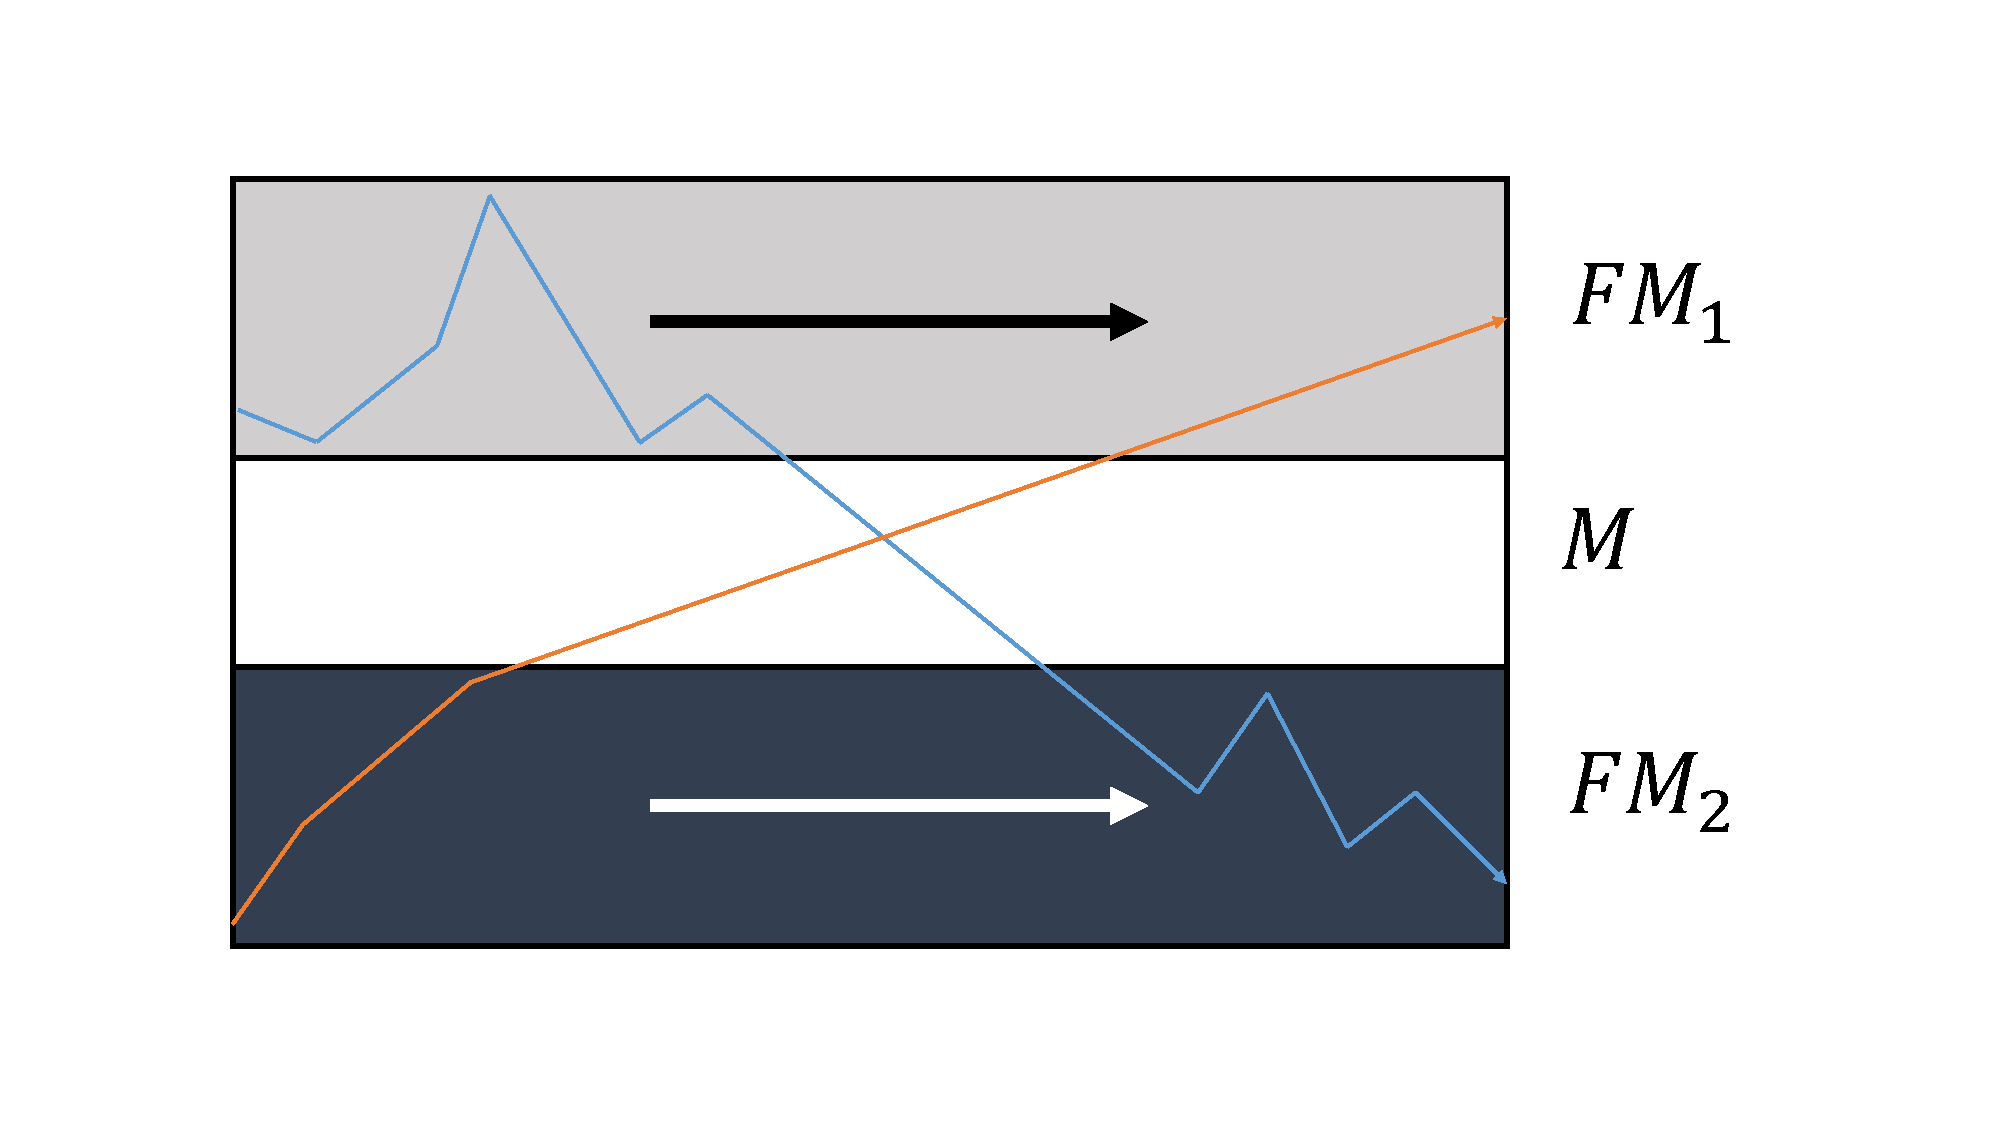
\includegraphics[width=\textwidth, page=1]{gmr_effect.pdf}
        \caption{Parallel ferromagnetic layers alignment.}
        \label{figure:gmr-effect-parallel}
    \end{subfigure}
    \hfill
    \centering
    \begin{subfigure}[b]{.49\textwidth}
        \centering
        \includegraphics[width=\textwidth, page=2]{gmr_effect.pdf}
        \caption{Antiparallel ferromagnetic layers alignment.}
        \label{figure:gmr-effect-antiparallel}
    \end{subfigure}
    \caption{Working principle of the GMR effect (adapted from Soares \textit{et al.} \protect\cite{Soares2019}).}
    \label{figure:gmr-effect}
\end{figure}

Figure \ref{figure:gmr-effect} shows the working principle of the \ac{GMR} effect using stacked layers. The effect occurs whether the magnetization of adjacent ferromagnetic layers is parallel alignment shown in Figure \ref{figure:gmr-effect-parallel} or antiparallel alignment shown in Figure \ref{figure:gmr-effect-antiparallel}. Among the various combination of materials used for forming these layers: Co, Fe, NiFe, CoFe and other alloys are used as ferromagnetic layers, while Cr, Cu, Ag, and others are used for the interlayer \cite{4463868}. In the first case, spin-down electrons have a higher scattering probability than the spin-up electrons creating a lower resistivity channel for spin-up electrons, which lowers the overall resistance of the device. In the second case, both the spin-up and spin-down electrons will have a high scattering probability in the respective ferromagnetic layer with opposite moments generating two channels with the same resistivity. The resistivity of this channel is higher than the low resistance channel of the first case, therefore producing an overall higher resistivity than the parallel state.

A \ac{GMR} stack is typically composed of several ferromagnetic and non-magnetic layers and has a magnetic response illustrated in Figure \ref{figure:mr-transfer-curves-b}. The $MR_{ratio}$ of these sensors can amount to 10\%.
% ----------------------------------------------------------------------------- Giant Magnetoresistance

% ----------------------------------------------------------------------------- Spin Valve Sensors
\mytitle{Spin Valve Sensors}

\noindent
A \ac{SV} sensor is a device in which the electrical resistance varies within the interval of two values. The \ac{SV} consists of two conducting magnetic materials (pinned and free layer) with different magnetic coercivities. The resistance change is a result of the \ac{GMR} effect.

In 1991 Dieny \textit{et al.} \cite{PhysRevB.43.1297} introduced the principle of an \ac{SV} sensor comprising a fixed ferromagnetic layer, called pinned layer, and another ferromagnetic layer free to rotate with the external field. This concept was further developed and tested in 1994 \cite{312279}. Nowadays, \ac{SV} sensors are used in magnetic sensors, hard disk read heads \cite{IBMResea24:online}, and magnetic random access memories.

\begin{figure}[!ht]
    \centering
    \begin{subfigure}[b]{.48\textwidth}
        \centering
        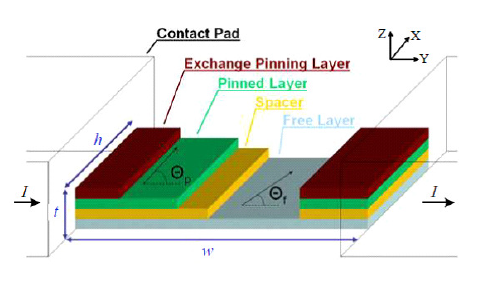
\includegraphics[width=\textwidth]{sv_structure.png}
        \caption{Simplied structure.}
        \label{figure:sv-structure}
    \end{subfigure}
    \hfill
    \centering
    \begin{subfigure}[b]{.48\textwidth}
        \centering
        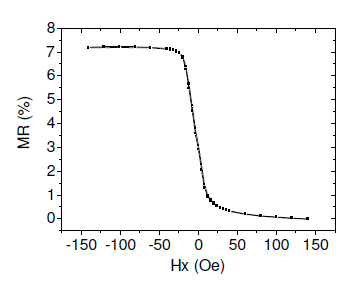
\includegraphics[width=.65\textwidth]{sv_experimental.png}
        \caption{Experimental transfer curve (MR characteristic).}
        \label{figure:sv-characteristic}
    \end{subfigure}
    \caption{SV sensor features (from \textit{Dr.} Tiago Costa \cite{TiagoC_thesis}).}
    \label{figure:sv-sensor}
\end{figure}

The simplified \ac{SV} sensors structure, illustrated in Figure \ref{figure:sv-structure}, consists of a copper spacer sandwiched between two ferromagnetic layers, one of which is fixed (pinned) by an antiferromagnet that raises the magnetic coercivity of that layer.

As outlined in the previous section, the electrical resistance is higher when the alignment of the magnetic layers is antiparallel than in parallel. The working principle is based on the \ac{GMR} phenomenon, and upon sensing a magnetic field with an appropriate strength, the free layer switches polarity, resulting in a resistance change shown in Figure \ref{figure:mr-transfer-curves-a}. When the maximum magnetic field is applied, the electron spin of both ferromagnetic layers are in the parallel state, and thus the \ac{SV} sensor resistance has its minimum value of $R_{min}$. When such a magnetic field is applied that causes the electron spin of both ferromagnetic layers to be in the
anti-parallel state, the \ac{SV} sensor resistance reaches its maximum value $R_{max}$. Between these two states, the \ac{SV} sensor resistance has a linear response with the applied magnetic field \cite{TiagoC_thesis}.


Freitas \textit{et al.} \cite{freitas2007magnetoresistive} fabricated several \ac{SV} sensors with different ferromagnetic materials and thicknesses and reported up to 20\% $MR_{ratio}$. One of these sensors with a width of $\mathrm{6~\mu m}$ and height of $\mathrm{2~\mu m}$ was used to obtain the \ac{MR} characteristic illustrated in Figure \ref{figure:sv-characteristic}. These dimensions achieved a typical relative value for the $MR_{ratio}$ of around 7\%.
% ----------------------------------------------------------------------------- Spin Valve Sensors
% ############################################################################# Magnetoresistive Sensors

% ############################################################################# Sensor Front-End Interfaces
\section{Sensor Front-End Interfaces}
\label{section:soa-interfaces}

The \ac{MR} sensors are resistive sensors that change their resistance according to a magnetic field. To obtain these resistance values and translate them to meaningful information, an analog interface is fundamental to bias the sensors, amplify their signal and perform other required functions.

Over the last decades, the front-ends have benefited from technological advances to be a low-cost and versatile interface for resistive sensors offering both a wide operative range and robustness to component and power supply variations. The result is a simple, compact, low-cost, low-voltage and low-power solution \cite{electronics8030263}.

The type of resistance variation of the sensor follows two different paradigms. In the first measurement paradigm, the resistance variation of the sensors can last for several decades \cite{5938039}. Where the interface, depending on the type of application, must have: a high dynamic range and precision for the entire range \cite{5938039, 1465853}; a increased throughput for very high resistance values \cite{4099747}; temperature gradient control \cite{4124708}; auto-scaling scheme \cite{4114752}; reduced power consumption \cite{6330702}; among other features. The second measurement paradigm is related to the minimum detectable resistance variation that the interface can recognize for a given resistive sensor. The \ac{SV} sensors are a great example because they can measure weak magnetic fields and thus may produce signals with low intensities ($\mathrm{\mu V}$). Therefore, when designing a front-end interface for this type of sensor, it is crucial to ensure that the interface noise remains below the level of the sensor noise. This ensures that the \ac{SNR} is not compromised or diminished.

% ----------------------------------------------------------------------------- Work from Hall et al. at Stanford University
\subsection{Work from Hall \textit{et al.} at Stanford University}

The team Hall \textit{et al.} \cite{PMID24761029} were aware that the future of medical diagnostics lies within magnetic nanotechnologies. It has proven potential in several nanomedicine areas like imaging, therapeutics, and early disease detection. The advancements in nanotechnology promote new transducers with the same size scale as biomolecules, using electronic detection instead of the typical optical molecular tests. However, to achieve this end, novel biosensing interfaces are required to make this transition possible.

Hall \textit{et al.} project presents a quantitative platform that uses magnetic immunoassays coupled with an array of magnetic biosensors and an integrated data acquisition system. It performs high-sensitivity electronic molecular tests enabling quantitative proteomic analysis, following a similar working principle as the system in this dissertation by detecting with \ac{MR} sensors \ac{MNP} attached to the analytes.

\begin{figure}[!ht]
    \centering
    \begin{subfigure}[b]{.49\textwidth}
        \centering
        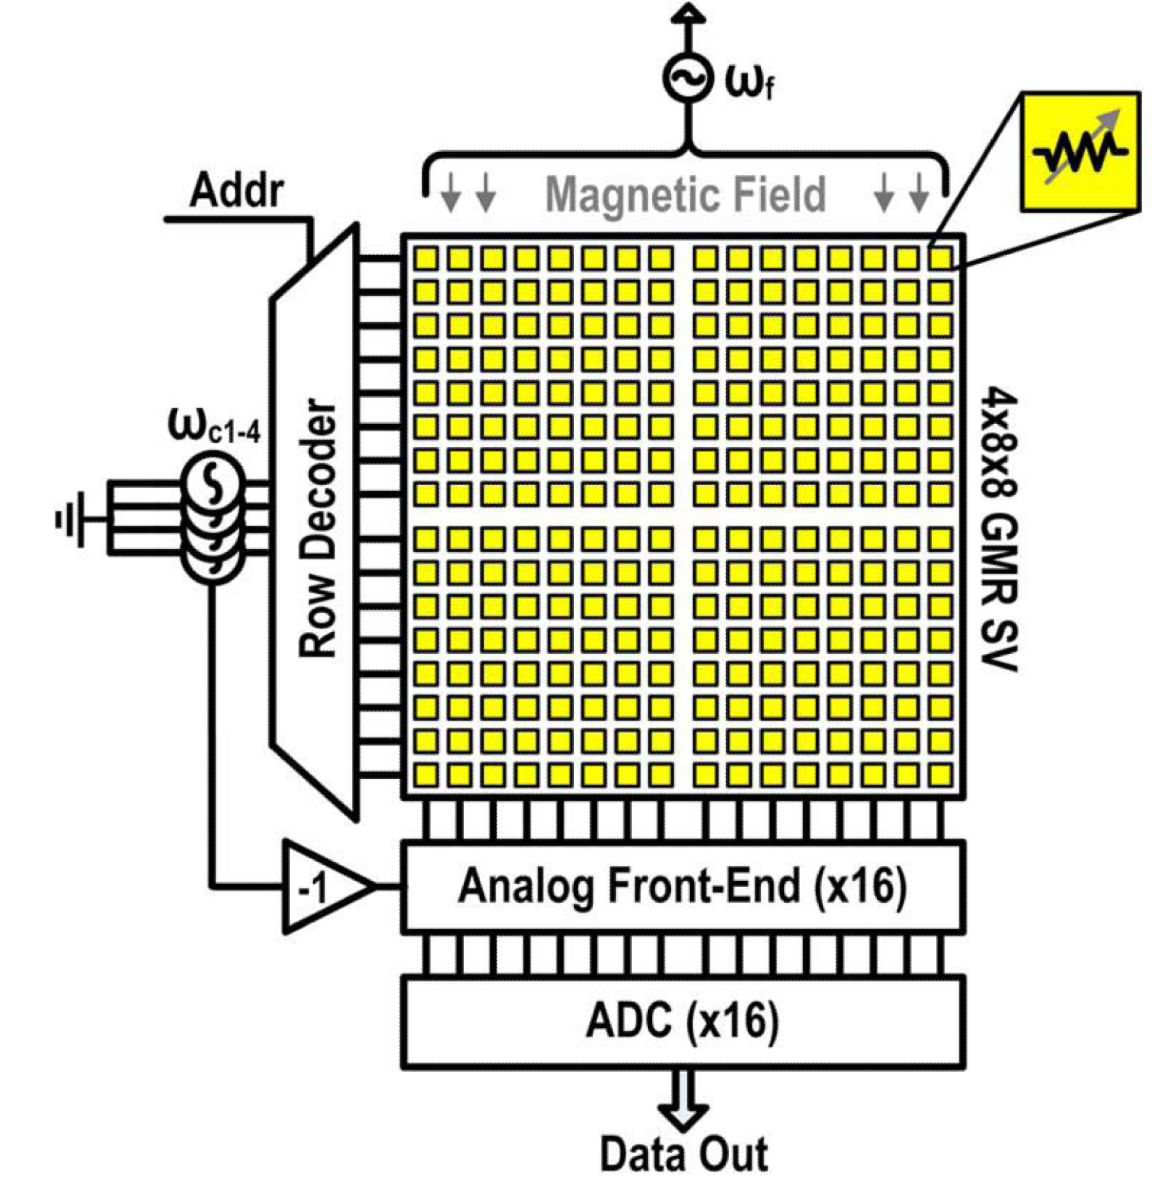
\includegraphics[width=.8\textwidth]{hall_et_al/hall_sensor_architecture.jpg}
        \caption{Architecture of the MR sensor system.}
        \label{figure:hall-sensor}
    \end{subfigure}
    \hfill
    \centering
    \begin{subfigure}[b]{.49\textwidth}
        \centering
        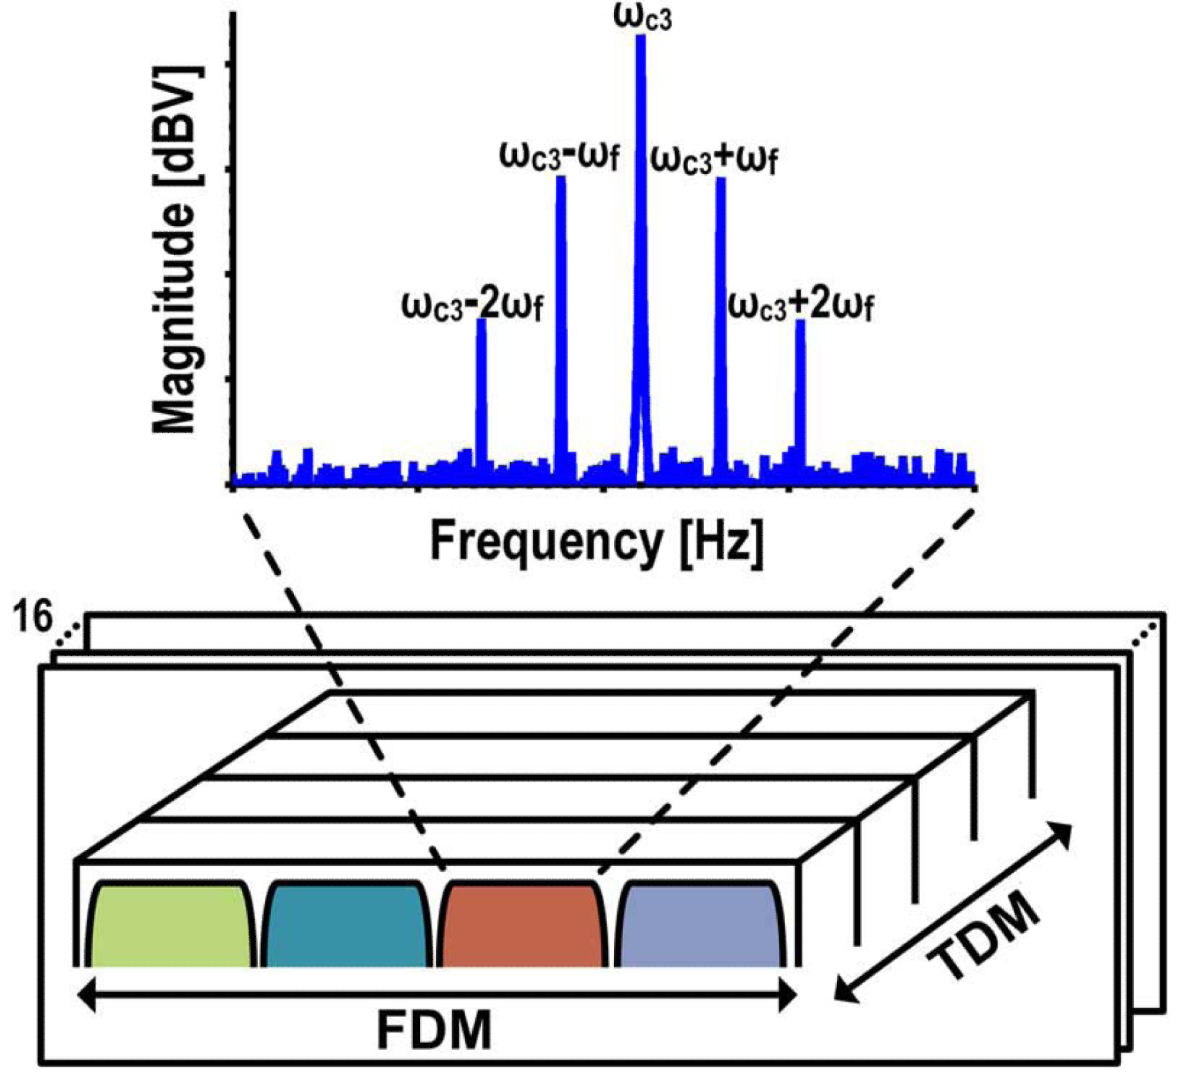
\includegraphics[width=.73\textwidth]{hall_et_al/hall_modulation.png}
        \caption{FDM spectrum and principle.}
        \label{figure:hall-modulation}
    \end{subfigure}
    \caption{SV sensor interface (from Hall \textit{et al.} \cite{PMID24761029}).}
    \label{figure:hall-sensor-interface}
\end{figure}

Figure \ref{figure:hall-sensor} depicts the organization of the \ac{MR} sensors within the interface, composed of four sub-arrays, each with an 8x8 \ac{2D} matrix of \ac{SV} sensors. The sensor array exceeds in mitigating the 1/f noise component of \ac{MR} sensors by modulating the signal and applying an \ac{AC} magnetic field ($w_f$) to excite the \ac{MNP}s and an \ac{AC} voltage ($w_{c_{1-4}}$) to bias the sensors. The system is composed of a decoder that selects a particular row of the sensors that are readout in parallel by column level \ac{ADC}s.

The sensor array has a total of 256 individually addressable sensors \ac{MR} sensors. Usually, in large arrays, \ac{TDM} is used to scan each sensor. However, this project uses 16 parallel readout channels and an \ac{FDM} to reduce the readout time due to the adopted signal modulation scheme. As shown in Figure \ref{figure:hall-modulation}, the \ac{FDM} is performed by biasing each of the four sub-arrays with a different carrier frequencies ($w_{c_{1-4}}$) and summing the resultant \ac{MR} sensor currents. The spectrum tone at $w_c$, the carrier tone, is due to the non-magnetoresistive portion of the sensor, whereas the side tones at $w_c \pm wf$ result from the magnetoresistive component. Additionally, the signal baseline ratio is improved by extracting the side tones (magnetoresistive component) of the signal.

\begin{figure}[!ht]
    \centering
    \begin{subfigure}[b]{.49\textwidth}
        \centering
        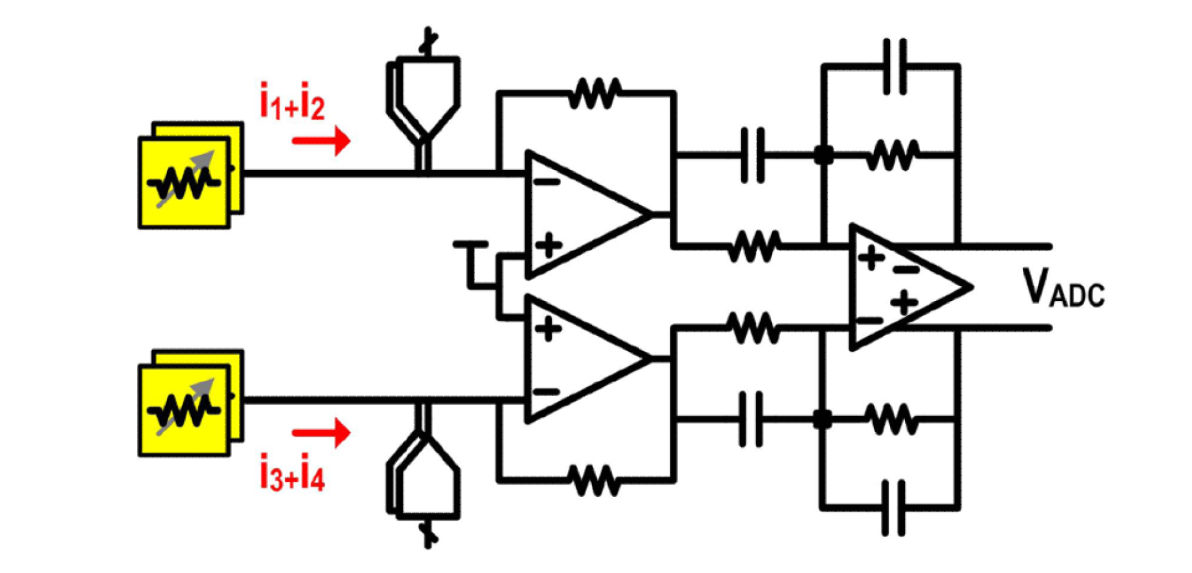
\includegraphics[width=.9\textwidth]{hall_et_al/hall_readout_channel.png}
        \caption{Readout channel with carrier suppression.}
        \label{figure:hall-readout-channel}
    \end{subfigure}
    \hfill
    \centering
    \begin{subfigure}[b]{.49\textwidth}
        \centering
        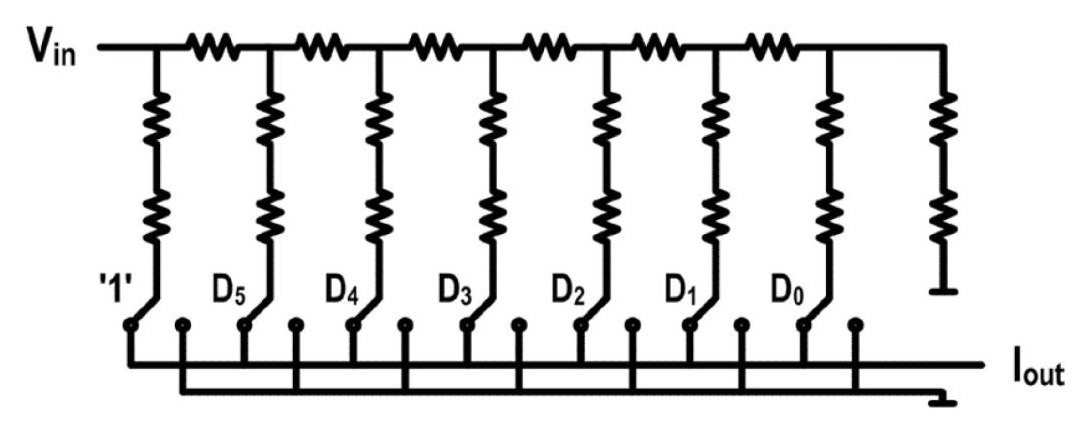
\includegraphics[width=.9\textwidth]{hall_et_al/hall_ladder.png}
        \caption{R-2R ladder for carrier suppression.}
        \label{figure:hall-ladder}
    \end{subfigure}
    \caption{Analog front-end schematic (from Hall \textit{et al.} \cite{PMID24761029}).}
    \label{figure:hall-afe}
\end{figure}

The \ac{AFE}, in Figure \ref{figure:hall-readout-channel}, is implemented by two differential \ac{TIA}s followed by a fully-differential \ac{ADC} driver. The split architecture optimizes each amplifier separately, using the \ac{TIA} low noise and high linearity and the high speed of the \ac{ADC} driver. The \ac{TIA}s process the current from two of the four sub-arrays and use a carrier suppression technique to increase the dynamic range. The four \ac{DAC}s at the input of each \ac{TIA}, corresponding to the four different carrier signals ($w_{c_{1-4}}$), attenuate the non-magnetoresistive component, which provides no information regarding the measurement. The \ac{DAC}s topology, depicted in Figure \ref{figure:hall-ladder}, is a $\mathrm{7\textnormal{-}bit}$ R-2R ladder with the most significant bit tied to logic one.

\begin{figure}[!ht]
    \centering
    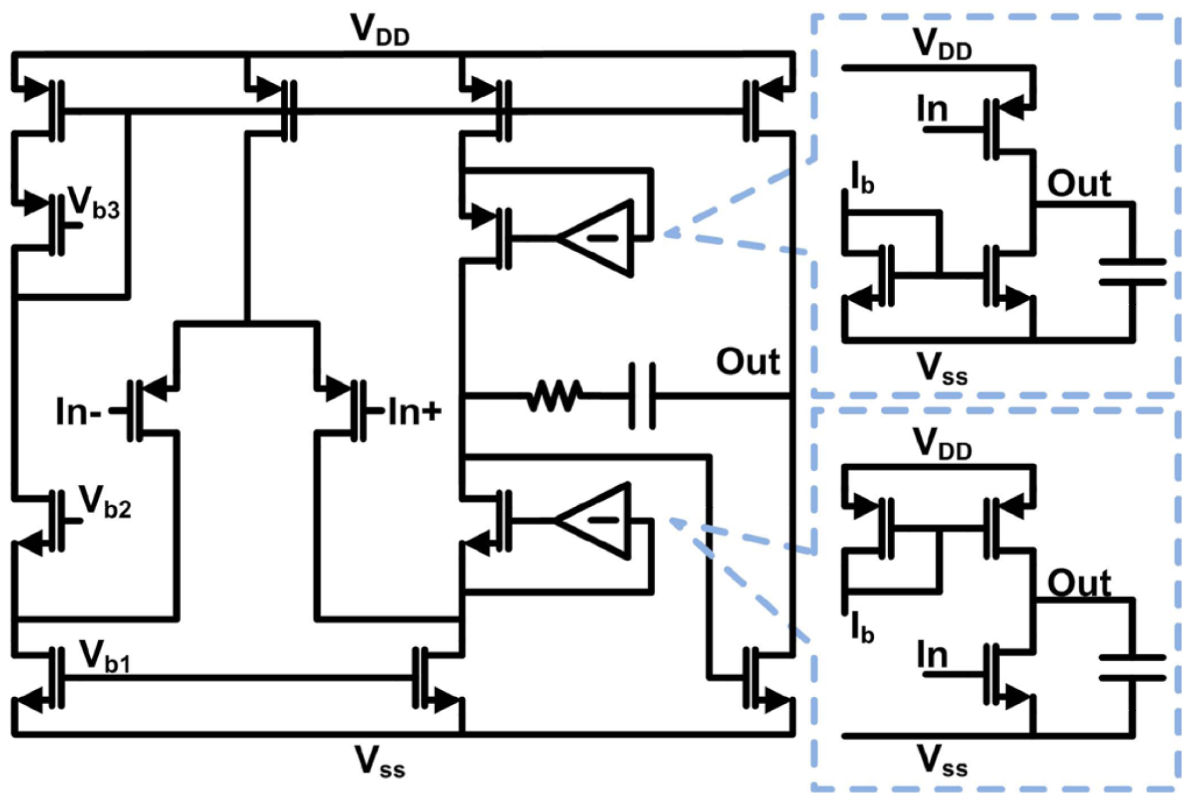
\includegraphics[width=.5\textwidth]{hall_et_al/hall_tia.jpg}
    \caption{Transimpedance amplification stage with carrier suppression and gain-boosters (from Hall \textit{et al.} \cite{PMID24761029}).}
    \label{figure:hall-tia}
\end{figure}

Figure \ref{figure:hall-tia} illustrates the schematic of a \ac{TIA}, implemented with a two-stage folded-cascode amplifier with gain-boosting and resistive feedback. The system uses pseudo-differential instead of fully-differentials \ac{TIA}s because it would add too much 1/f noise or require too much area. The closed-loop gain is established by resistive feedback, and the gain-boosters are implemented with common-source amplifiers.
% ----------------------------------------------------------------------------- Work from Hall et al. at Stanford University

% ----------------------------------------------------------------------------- Work from Germano et al.
\subsection{Work from Germano \textit{et al.}}

Germano \textit{et al.} \cite{Germano2006MICROSYSTEMFB} developed a microsystem for biomolecular recognition (e.g. enzymes) based on a biochip. The biochip follows the same principle of this project. It uses high sensitivity sensors to detect magnetically tagged biomolecules. The microsystem provides the electronic circuitry to address and read the \ac{MR} sensors, based on an \ac{MTJ}, organized in a \ac{2D} array. The developed prototype (Figure \ref{figure:germano-prototype}) with credit card dimensions has all the required electronics to address, read and sense the sensors, besides controlling the temperature and the microfluidics chamber.

\begin{figure}[!ht]
    \centering
    \begin{subfigure}[b]{.48\textwidth}
        \centering
        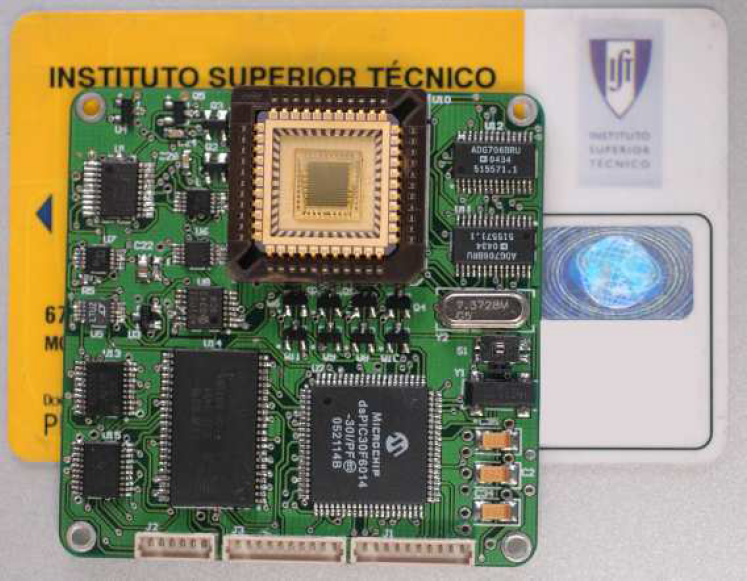
\includegraphics[width=.9\textwidth]{germano_et_al/germano_prototype.png}
        \caption{Prototype: main board.}
        \label{figure:germano-prototype}
    \end{subfigure}
    \hfill
    \centering
    \begin{subfigure}[b]{.48\textwidth}
        \centering
        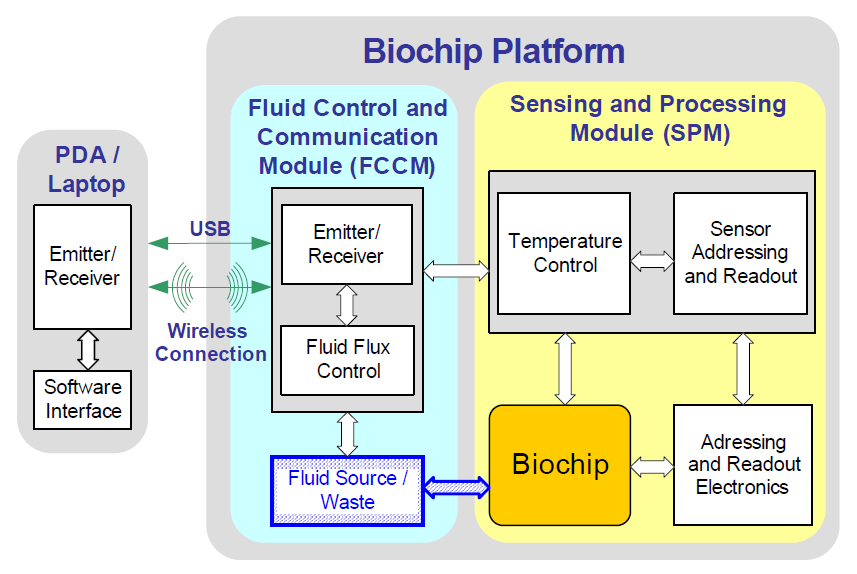
\includegraphics[width=\textwidth]{germano_et_al/germano_platform_architecture.png}
        \caption{Platform architecture.}
        \label{figure:germano-architecture}
    \end{subfigure}
    \caption{Microsystem for biological analysis (from Germano \textit{et al.} \cite{Germano2006MICROSYSTEMFB}).}
    \label{figure:germano-system}
\end{figure}

The platform architecture, depicted in Figure \ref{figure:germano-architecture}, is organized into two main modules: the sensing and processing module; and the fluid control and communications module. The first module directly interacts with the array of biosensors. It is responsible for addressing and reading the sensors and monitoring the temperature in different sub-areas of the chip. The second module, fluid control and communications, is the interface between the external world and the biochip platform. The architecture is flexible and reliable, including wired (\ac{USB} protocol) and wireless (Bluetooth technology) communication. This module also controls the fluid that carries the magnetically tagged biomolecules. The interface between the user and the portable system is through a handheld analyzer that allows a user-friendly interaction and provides the performed biological measures.

Since the \ac{MTJ} sensors are passive elements, they require a biasing structure to supply the necessary current. The current generator circuit in the biochip uses a \ac{DAC} and a voltage-to-current converter, as demonstrated in Figure \ref{figure:germano-bias}.

\begin{figure}[!ht]
    \centering
    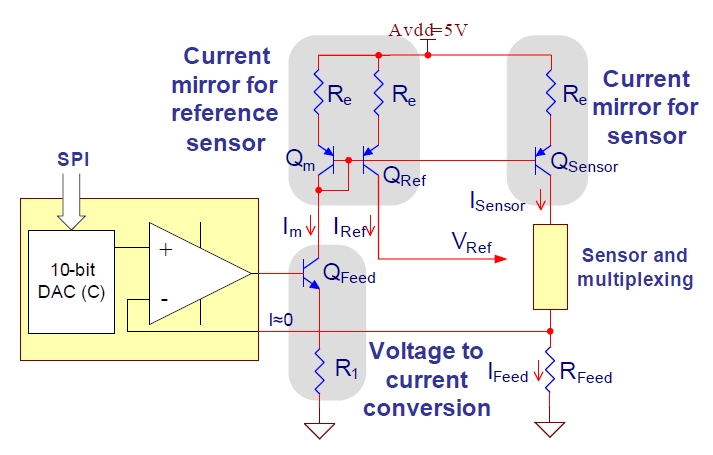
\includegraphics[width=.55\textwidth]{germano_et_al/germano_bias.png}
    \caption{Current generation circuit (from Germano \textit{et al.} \cite{Germano2006MICROSYSTEMFB}).}
    \label{figure:germano-bias}
\end{figure}

The output voltage of the 10-bit \ac{DAC} is converted to current, through a non-inverting amplifier topology, with a \ac{BJT} ($Q_{feed}$) and a resistor ($R_1$). The current mirror assures that the converted current injected into the sensor and the reference sensor has equal value. The degenerated current mirror replicates the same current value through the different branches if the degenerating resistances ($R_e$) have the same value. These $R_e$ resistances also introduces negative series-series feedback and increase the circuit output impedance improving the circuit operation. This topology reduces the current errors introduced by the current mirror and the feedback transistors, but the offset error of the op-amp remains.

The \ac{MR} sensors arranged in a \ac{2D} array (16x16) are addressed based on a multiplexer and a commutating matrix of integrated diodes, acting as a switch. The microcontroller is responsible for addressing a single element, providing the row and column of the desired sensor to be read. The addressing requires two multiplexers (row and column) to establish a single current path that includes the demanded sensor. Figure \ref{figure:germano-addressing} depicts the explained addressing architecture.

\begin{figure}[!ht]
    \centering
    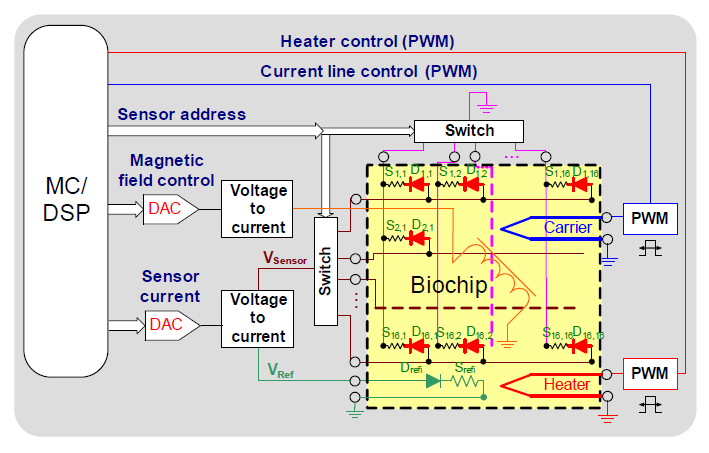
\includegraphics[width=.55\textwidth]{germano_et_al/germano_addressing.png}
    \caption{Addressing and sensor drive (from Germano \textit{et al.} \cite{Germano2006MICROSYSTEMFB}).}
    \label{figure:germano-addressing}
\end{figure}

The biochip also included several heaters placed in different chip areas to control the temperature using \ac{PWN} signals. It also has carrier lines to guide the target biomolecules over the magnetic sensor. The signal response of the \ac{MR} sensors can be measured by reading the voltage drop at $V_{sensor}$ in Figure \ref{figure:germano-addressing}. This voltage is measured using the conditioning circuit in Figure \ref{figure:germano-read}.

\begin{figure}[!ht]
    \centering
    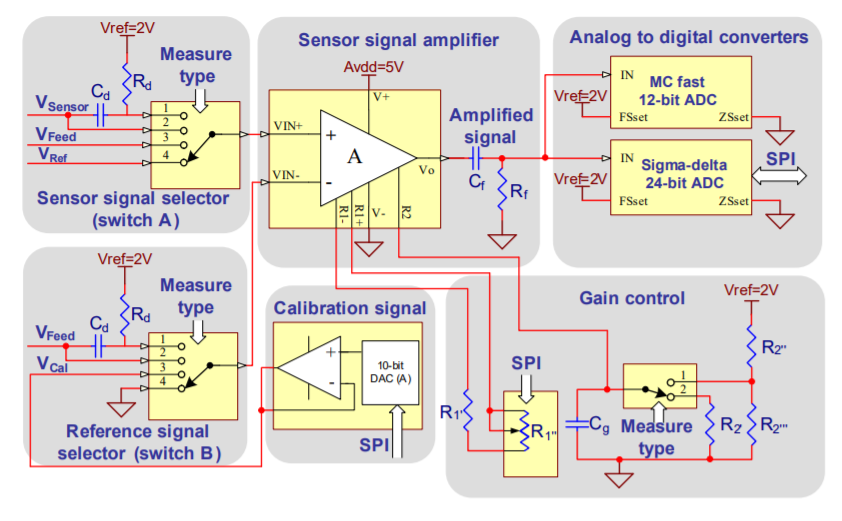
\includegraphics[width=.55\textwidth]{germano_et_al/germano_read.png}
    \caption{Circuit diagram of the sensor reading (from Germano \textit{et al.} \cite{Germano2006MICROSYSTEMFB}).}
    \label{figure:germano-read}
\end{figure}

Figure \ref{figure:germano-read} illustrates the diagram of the sensor readouts. The signals connected to the amplifier stage are defined using two switches. This circuit can provide several measurement types, including calibration measurements, with two different resolutions/speeds and controllable gain \cite{Germano2006MICROSYSTEMFB}.

The amplified signal is converted to the digital domain with a sigma-delta converter or a faster successive approximation \ac{ADC}. The signal information is transmitted to the microcontroller through a serial peripheral interface. The gain control circuit controls the sensor's temperature by adjusting the amplifier gain stage and, therefore, the sample acquisition time.
% ----------------------------------------------------------------------------- Work from Germano et al.

% ----------------------------------------------------------------------------- Work from Costa et al.
\subsection{Work from Costa \textit{et al.}}

The research team, Costa \textit{et al.} \cite{TIM.2013.2296417},  developed a neural signal detector for biologically generated magnetic fields. The system purpose is to record the magnetic field generated by ionic currents. It measures the voltage generated by the flow of ionic currents due to neuronal interactions \cite{4545308}, providing valuable information regarding how neurons interact. The system electronics include an ultra-low noise \ac{DC} or/and \ac{AC} source to bias the \ac{MR} sensors and the amplification and filtering circuit for the resulting signal.

Figure \ref{figure:costa-prototype} represents the prototype of the instrumentation system used in this project. The system includes three different boards: the current source and pre-amplifier, variable gain amplifiers and filters, and control board. The current source and the pre-amplifier provide the necessary current for the \ac{MR} sensors to generate a weak amplified signal in response to the neuronal signal. The variable gain amplifiers and filters perform the remaining amplification and remove unwanted components. The control boards allow for a manual configuration of the amplifiers and filters of the system.

\begin{figure}[!ht]
    \centering
    \begin{subfigure}[b]{.48\textwidth}
        \centering
        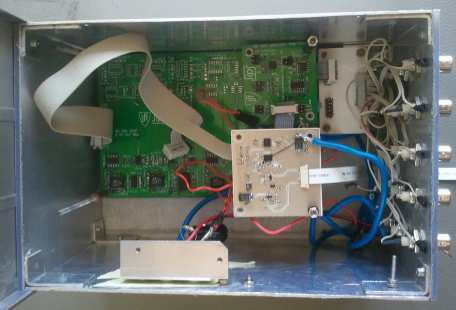
\includegraphics[width=\textwidth]{costa_et_al/costa_prototype.jpg}
        \caption{Instrumentation system prototype.}
        \label{figure:costa-prototype}
    \end{subfigure}
    \hfill
    \centering
    \begin{subfigure}[b]{.48\textwidth}
        \centering
        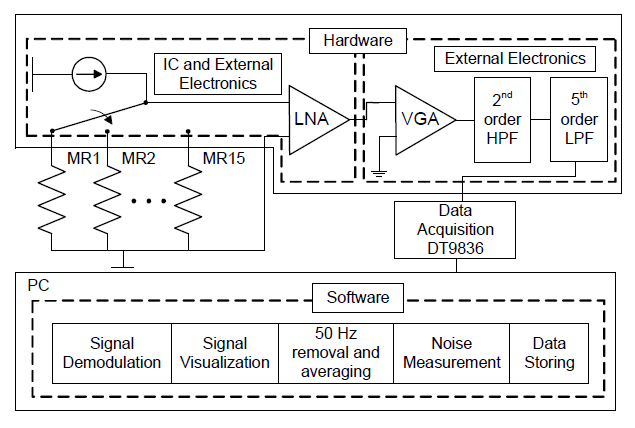
\includegraphics[width=\textwidth]{costa_et_al/costa_architecture.png}
        \caption{Block diagram of the system architecture.}
        \label{figure:costa-architecture}
    \end{subfigure}
    \caption{Neuronal signal detector for biological generated magnetic fields (from Costa \textit{et al.} \cite{TIM.2013.2296417}).}
    \label{figure:costa-system}
\end{figure}

The instrumentation system follows the architecture presented in Figure \ref{figure:costa-architecture} by a block diagram. The system is composed of hardware and software parts. Although, only hardware, the pertinent topic in the scope of this dissertation, will be approached in detail. The developed front-end includes a current source to bias the \ac{MR} sensors and an ultra-low noise \ac{AC} coupled instrumentation amplifier to intensify the signal response of the sensors. Furthermore, it has a variable gain amplifier, a 2\textsuperscript{nd} order \ac{HPF} and a 5\textsuperscript{th} order \ac{LPF} to amplify and limit the measurement bandwidth. The analog data is converted to digital using an \ac{ADC}, and it is the channel between the interface and the computer with the software implemented in MATLAB. The software allows the visualization and storage of the measurement signals.

The neuronal measurement with the \ac{MR} sensor follows this principle. A brain slice stimulated with an electrode generates action potentials due to neuronal activity at the tissue surface. These action potentials lead to ionic currents that produce magnetic fields. The \ac{MR} sensors detect this magnetic field, and the measurement is performed by biasing the sensors with a current and converting their resistance change into a voltage. However, the capacitive coupling between the brain and the \ac{MR} sensors induce an undesired voltage that masks the signal generated in response to the ionic currents. Biasing the sensors with a \ac{DC}+\ac{AC} current enables an amplitude modulation scheme that distinguishes the coupling voltage. The voltage variation due to neuronal magnetic interaction will appear in the baseband and around a specific frequency, whereas the coupling voltage is only present in the baseband.

The biasing current source, presented in Figure \ref{figure:costa-bias}, is based on a typical voltage regulator structure with negative feedback with a current output. A voltage \ac{DC} or \ac{DC}+\ac{AC} is applied to the ultra-low noise amplifier ($amp_c$) that, due to negative feedback, ensures the current $I_B$, and the voltage drop on $R_{REF}$ equals $V_B$. As mentioned before, to filter the coupling voltage, the $V_B$ voltage must have an \ac{AC} component generated by the circuit in Figure \ref{figure:costa-oscillator}. The schematic represents a typical Wien bridge oscillator, using a low noise rail-to-rail amplifier. This type of oscillator is known for having a \ac{BPF} (\ac{HPF} followed by \ac{LPF}) \ac{RC} network in the feedback loop. A buffered voltage divider from the power supply generates the voltage $V_{REF}$.

\begin{figure}[!ht]
    \centering
    \begin{subfigure}[b]{.49\textwidth}
        \centering
        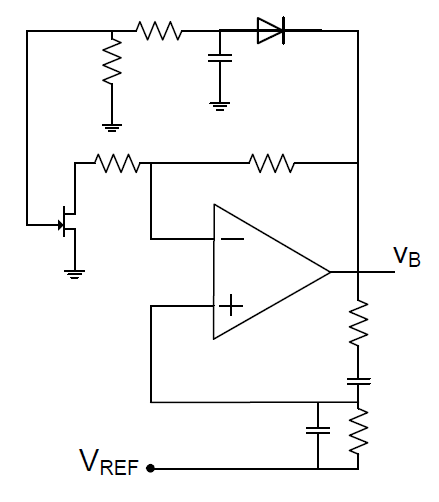
\includegraphics[width=.73\textwidth]{costa_et_al/costa_oscillator.png}
        \caption{Wien bridge oscillator for DC+AC current generation.}
        \label{figure:costa-oscillator}
    \end{subfigure}
    \hfill
    \centering
    \begin{subfigure}[b]{.49\textwidth}
        \centering
        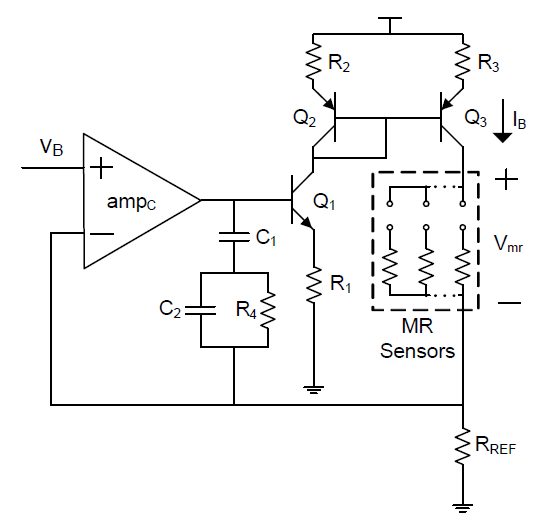
\includegraphics[width=.9\textwidth]{costa_et_al/costa_biasing.png}
        \caption{MR sensor biasing current source.}
        \label{figure:costa-bias}
    \end{subfigure}
    \caption{Biasing schematic (from Costa \textit{et al.} \cite{TIM.2013.2296417}).}
    \label{figure:costa-bias-schematic}
\end{figure}

Figure \ref{figure:costa-amp} depicts the amplification and filtering block diagram. The amplification has two stages, an ultra-low noise instrumentation amplifier ($\mathrm{AD8429}$) and a variable gain instrumentation amplifier ($\mathrm{AD8231}$). The typical neuronal signal is in the $\mathrm{\mu V}$ range. However, it can have a higher amplitude. The 2\textsuperscript{nd} stage amplifier has a variable gain to prevent system saturation. The 1\textsuperscript{st} stage amplifier is an ultra-low noise to decrease the next stage impact on the \ac{SNR} of the measurement. The 2\textsuperscript{nd} order \ac{HPF} ($\mathrm{LMF100}$) reduces the flicker noise, whereas the 5\textsuperscript{th} order \ac{LPF} reduces the high-frequency noise.

\begin{figure}[!ht]
    \centering
    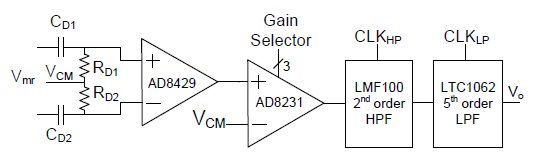
\includegraphics[width=.7\textwidth]{costa_et_al/costa_amp_n_filt.png}
    \caption{Variable gain amplifier and bandpass filter block diagram (from Costa \textit{et al.} \cite{TIM.2013.2296417}).}
    \label{figure:costa-amp}
\end{figure}

Neuronal applications such as this one require a measurement system with a high spatial resolution. The instrumentation system described can measure signals from a maximum of 16 sensors if there are 16 current sources designed. Hence, the research team from \ac{INESC} is developing new biasing and amplification circuit to allow scaling the number of sensors. The enhancement of the system with a high spatial resolution, and immunity to external interference's, is being pursued to tolerate high-density neuronal measurements.
% ----------------------------------------------------------------------------- Work from Costa et al.

% ----------------------------------------------------------------------------- Work from Caetano et al.
\subsection{Work from Caetano \textit{et al.}}

This dissertation purpose is to improve the system implemented by the Caetano \textit{et al.} research team. The work disclosed in this sub-section is developed on top of previous efforts done by a multidisciplinary research team from \ac{INESC-MN} and \ac{INESC-ID}. This team was composed of Dr. Diogo Caetano, Eng. Rita Soares, and Eng. Ruben Afonso.

% --- Ruben --- 

\begin{figure}[!ht]
    \centering
    \begin{minipage}{0.38\textwidth}
        \centering
        \includegraphics[width=\textwidth, angle=270]{images/chapter_2/caetano_et_al/old_cyto.png}
        \caption{Cytometer platform designed by Eng. Ruben Afonso.}
        \label{figure:ruben-cyto}
    \end{minipage}\hfill
    \begin{minipage}{0.58\textwidth}
        \centering
        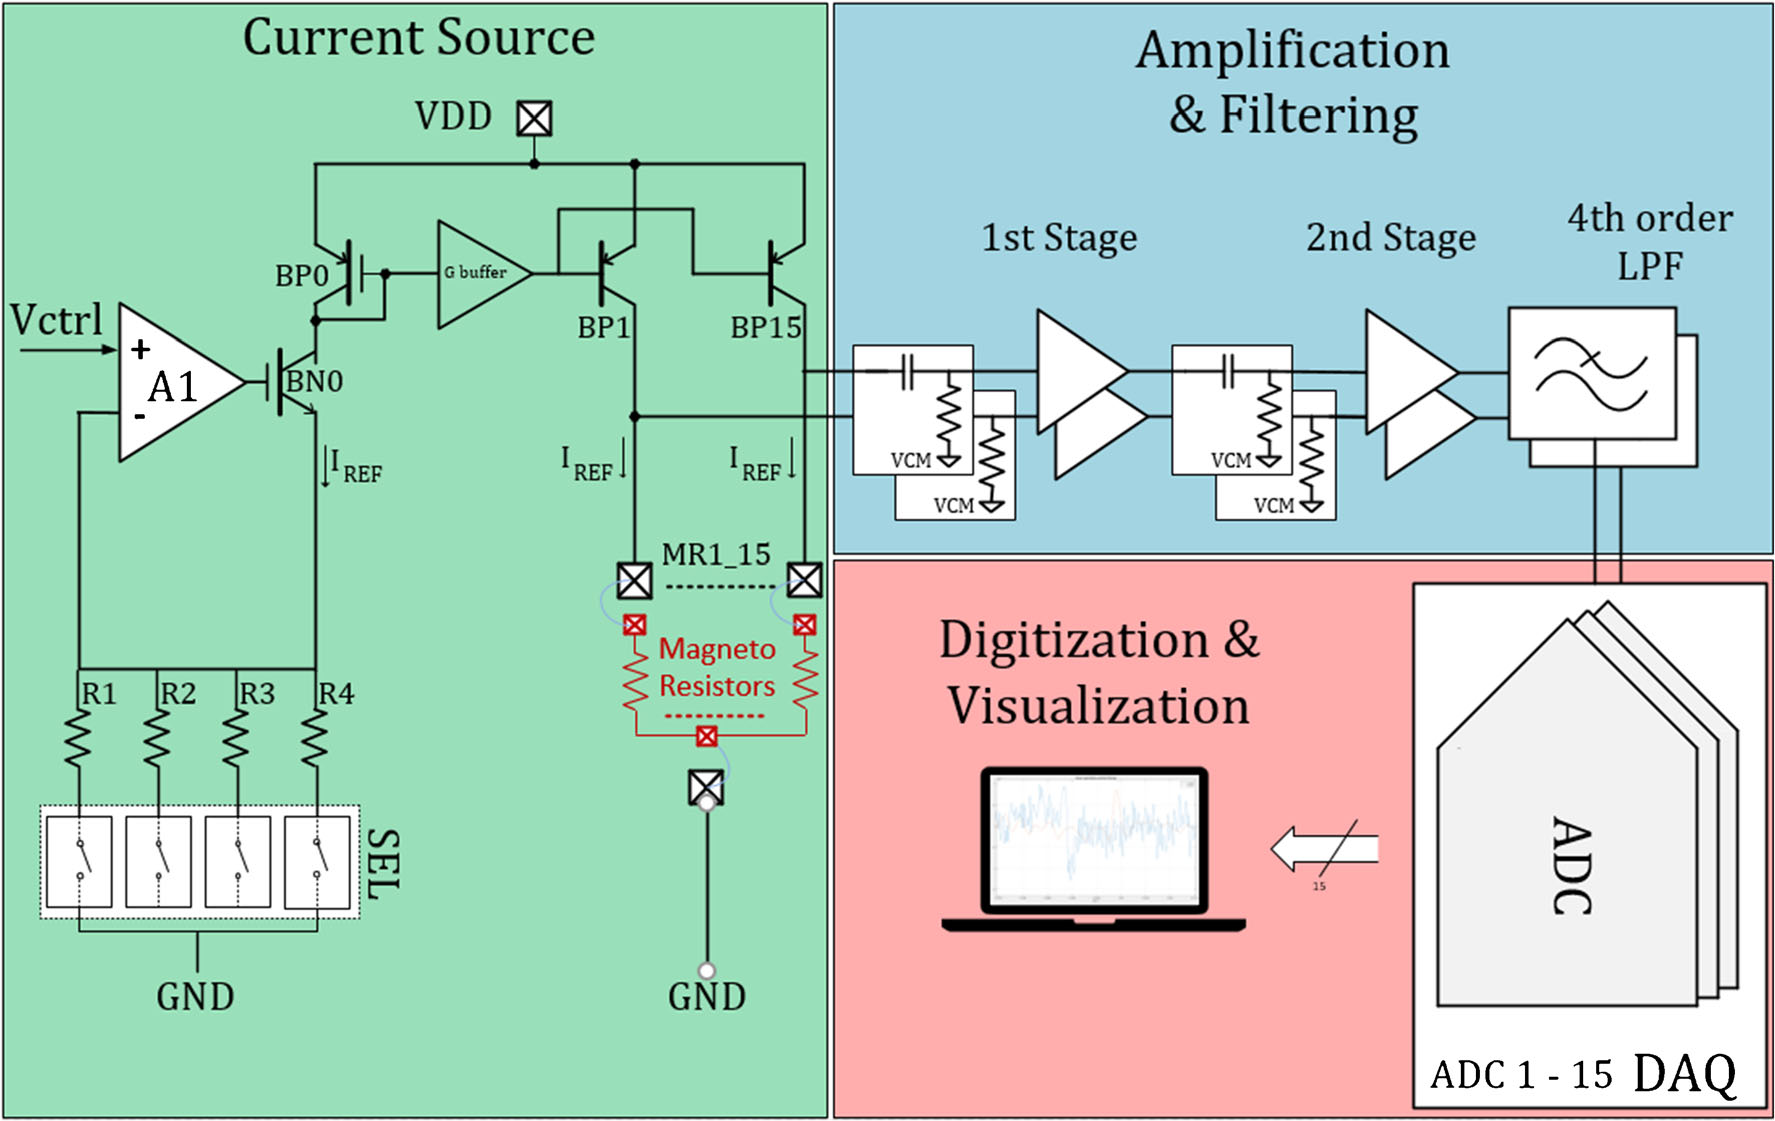
\includegraphics[width=\textwidth]{caetano_et_al/caetano_system.jpg}
        \caption{Schematic representation of the electronics for sensor biasing and signal acquisition used in MFC experiments (from Soares \textit{et al.} \cite{Soares2019}).}
        \label{figure:caetano-schematic-mfc}
    \end{minipage}
\end{figure}

The system for the \ac{MFC}, presented in Figure \ref{figure:caetano-schematic-mfc}, consists of three main sections: sensor biasing, signal amplification, and digitalization. In the biasing section, the output of the amplifier ($A_1$), established by a control voltage ($V_{crtl}$), is converted to current through the transistor $B_{N_0}$ and the $R_{1-4}$ resistances. The current mirror, performed by $B_{P_0}$ and $B_{P_{1-15}}$, assures that the converted current injected into all the sensors has the same value ($I_{ref}$). The signal amplification and filtering section comprise two \ac{AC} coupled amplification stages followed by a 4\textsuperscript{th} order anti-aliasing \ac{LPF}. This section takes the most space out of the board because each \ac{MR} sensor requires signal amplification and filtering circuitry. The digitalization section uses a \ac{DAQ} board, limiting the number of sensors to 15, which digitizes and multiplexes the analog inputs and allows to store the signal in a computer. Dr. Diogo Caetano also developed a script to process the raw signal data. The conceived script consisted of additional signal filtering, signal subtraction between a reference sensor with mismatch estimation, and the application of heuristics to select candidates to be identified by a machine learning algorithm.

Figure \ref{figure:ruben-cyto} showcases the current \ac{MFC} platform developed by Eng. Ruben Afonso. This board features two analog channels consisting of a biasing architecture with an open-loop topology and an amplification scheme. The analog channels were meticulously designed using discrete electronic components selected specifically for their intended purpose. In addition to the analog channel, the board incorporates a saturation detector in the 1\textsuperscript{st} stage of amplification and a power supervisor circuit. However, the saturation detector does not perform as expected when the saturation time is short. Eng. Ruben Afonso also designed two additional \ac{PCB}s that can be attached to the platform: one for the detection of magnetic field changes using \ac{SV} sensors, and another for \ac{DAQ} purposes. Overall, Afonso's work has yielded a compact and modular system.

Caetano's work was perfomed on the previously explained prototypes, consists of techniques to interface the \ac{MR} sensors. The developed and designed techniques improve the extraction of reliable information according to the specific application in the scope of biomolecular recognition. The developed \ac{AFE} consists of an adapted architecture from Germano \textit{et al.} \cite{Germano2006MICROSYSTEMFB} built on a platform implemented by Costa \textit{et al.} \cite{TIM.2013.2296417}. \textit{Dr.} Diogo Caetano work is focused on an \ac{AFE} for non-destructive tests and the digital signal processing for the \ac{MFC}.

\begin{figure}[!ht]
    \centering
    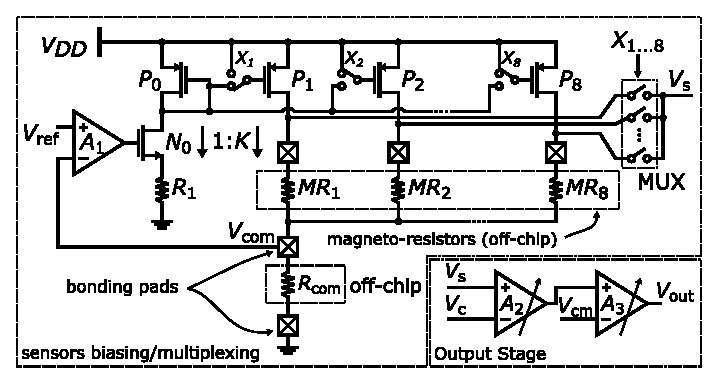
\includegraphics[width=.8\textwidth]{caetano_et_al/caetano_ndt.eps}
    \caption{Schematic representation of the electronics for sensor biasing and simplified output stage used in non-destructive tests experiments (from Dr. Diogo Caetano \cite{DiogoC_thesis}).}
    \label{figure:caetano-schematic-ndt}
\end{figure}

The biasing topology, shown in Figure \ref{figure:caetano-schematic-ndt}, used in the non-destructive tests system, has a similar working methodology as the previous system (Figure \ref{figure:caetano-schematic-mfc}). The interface bias the sensors with current and reads their response in voltage. The biasing current, controlled externally by $V_{ref}$, is converted to current with the transistor $N_0$ and the resistance $R_1$. The current mirror feeds all the sensors with the same current value. To do so, the transistor $P_0$ converts the current back to voltage, and the transistors $P_{1-8}$ convert the voltage into current to mirror it to all sensor branches. The \ac{MR} sensors change their resistance proportional to a magnetic field, resulting in the $V_s$ voltage signal. The sensors are addressed individually using a multiplexer controlled by the inputs $X_{1-8}$. The major difference between Figure \ref{figure:caetano-schematic-mfc} and Figure \ref{figure:caetano-schematic-ndt} systems is the feedback loop. Non-destructive tests system has sensors inside the feedback loop (closed-loop). Unlike the \ac{MFC} system, which is an open-loop with the sensors outside the feedback loop. The closed-loop approach provides an improvement in the noise, as most of the noise introduced by the circuitry is reduced by the amplifier. However, the disadvantage of this loop methodology is that it is more difficult to stabilize.
% ----------------------------------------------------------------------------- Work from Caetano et al.
% ############################################################################# Sensor Front-End Interfaces

% ############################################################################# Discussion
\section{Discussion}

In this chapter, the concept of \ac{MR} sensors was explored, specifically focusing on \ac{SV} sensors, which will be utilized in this project. \ac{MR} sensors are designed to detect and measure changes in magnetic fields by utilizing the magneto-resistive effect. Several platforms have been developed to interface with \ac{MR} sensors, enabling accurate and reliable measurements. By leveraging the advancements in \ac{MR} sensor technology and the design of these interface platforms, this work aims to achieve a precise and efficient magnetic field detection and measurement system.

\ac{MR} sensor is a broad term for devices designed to sense magnetic fields. Their resistance value change in the presence of a magnetic field. This project will take advantage of \ac{SV} sensors that are based on the \ac{GMR} effect. In the comprehensive review by the \ac{INESC-MN} research team (Soares \textit{et al.} \cite{Soares2019}), out of the thirty-one related works: twenty used \ac{GMR} sensors (\ac{SV} and \ac{GMR} stacks); four used hall sensors; and six used \ac{TMR}, coils, or giant magneto impedance sensors. The multilayers \ac{GMR} sensors have the best compromise between noise, signal, and fabrication simplicity. Another important feature when developing an interface for them is the ease of biasing and obtaining their response, either in \ac{AC} or \ac{DC} mode. To support this, \textit{Dr.} Diogo Caetano's work \cite{DiogoC_thesis} compared the \ac{SV} sensors with the \ac{MTJ}, which use the \ac{TMR} effect. On the one hand, he concluded that in noisy environments, \ac{MTJ}s tend to perform better \cite{s120912169, 8526523, ECNDT2014, sergeeva} as they produce more signal per unit of field but have a more considerable noise. On the other hand, in very low-signal and low-noise applications, \ac{SV}s generate less noise, so they are used more often \cite{Freitas2017SpintronicBF, C0LC00324G, Soares2019, 8379352, j.bios.2018.02.046}. In summary, it is clear that biomolecular recognition applications are driving \ac{SV} sensors development. Yet, there is also a growing number of other applications, such as flow cytometry, neuronal magnetic recording and non-destructive tests based on eddy current.

The \ac{AFE} interfaces are crucial to obtain the resistance change in the \ac{MR} sensors and translate them to meaningful information according to the application. Usually, the interfaces integrate the full analog path, from sensor biasing to signal digital conversion. Nevertheless, noise is one of the fundamental considerations, common through all interfaces that serve different applications. It is clear that \ac{MR} sensors have a huge potential in several applications, but it is crucial to develop ultra-low noise interfaces according to the application specifications. This chapter detailed four \ac{AFE} prototypes, three of them conceived in \ac{INESC}. The interfaces that Hall \textit{et al.} \cite{PMID24761029} and Germano \textit{et al.} \cite{Germano2006MICROSYSTEMFB} created were within the scope of biomolecular recognition applications. As opposed to Costa \textit{et al.} \cite{TIM.2013.2296417} and Caetano \textit{et al.} \cite{Soares2019, DiogoC_thesis}, which focused on flow cytometry applications. 

The examination of these cutting-edge prototypes has provided valuable insights for this thesis. Germano \textit{et al.} work introduced an intriguing concept of utilizing a \ac{DAC} to supply the reference voltage required by the biasing architecture. This concept allows for a easy adjustment of the biasing current without electronic expertise. This feature is particularly advantageous for this multidisciplinary project. Moreover, Dr. Tiago Costa, followed by Dr. Diogo Caetano, initiated studies on a novel biasing topology where the sensors are placed inside the feedback loop. This innovative topology holds the potential to significantly reduce the noise introduced by the cytometer platform. Eng. Ruben Afonso laid the groundwork for the \ac{MFC} system using discrete electronics. However, there is still room for improvement in the current system. To address this, the work presented in this thesis aims to develop an enhanced version of the system with additional debugging tools for comprehensive analysis and optimization.
% ############################################################################# Discussion

\clearpage
\thispagestyle{empty}
\cleardoublepage